% ----------------------------------------------------------
\chapter{DESENVOLVIMENTO} \label{cap:desenvolvimento}
% ----------------------------------------------------------

% A estrutura de seções deste capítulo varia em função das características de cada trabalho, e deve ser definida junto com o orientador no decorrer da disciplina. A seguir é apresentada uma estrutura de seções tradicionalmente utilizada em TCCs que envolvem o desenvolvimento de um software. 


% ----------------------------------------------------------
% \section{VISÃO GERAL DO PROJETO}\label{sec:visao}
% % ----------------------------------------------------------

% Em alguns casos, pode ser interessante fornecer ao leitor uma visão geral do projeto, especialmente quando a solução é complexa e/ou envolve diversos componentes. Você também pode utilizar esta seção para falar um pouco sobre o modelo de processo de software adotado (cascata, espiral, incremental, …) e o planejamento das atividades realizadas.

% \begin{figure}[htb]
% 	\begin{center}
% 		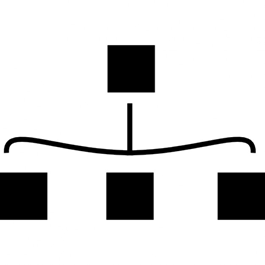
\includegraphics{images/figura1.png}
% 	\end{center}
% 	\caption{\label{fig:Fig_1}Visão geral do projeto}
% 	\fonte{Elaborado pelo autor deste trabalho (2018).}
% \end{figure}

% A Figura \ref{fig:Fig_1} representa ...

% ----------------------------------------------------------
% \section{LEVANTAMENTO DE REQUISITOS} \label{sec:requisitos}
% ----------------------------------------------------------

% Você pode iniciar esta seção explicando como e quando foram levantados os requisitos do sistema. Entrevistas com os proprietários da empresa? Documentação do software legado? Questionários aplicados aos usuários?

% Em seguida você deve apresentar a especificação dos Requisitos Funcionais, Requisitos Não Funcionais e Regras de Negócio do sistema, conforme os ensinamentos da disciplina de Engenharia de Software, por exemplo:

% A partir das entrevistas com os proprietários da empresa, foram identificados os seguintes requisitos funcionais para o sistema a ser desenvolvido:

% \textbf{RF01} – O sistema deverá permitir ao usuário manter produtos;

% \textbf{RF02} – O sistema deverá permitir ao usuário administrador manter categorias de produtos;

% \textbf{RF03} – ...

% Os seguintes requisitos não funcionais:

% \textbf{RNF01} – Todas as funcionalidades serão executadas online, ou seja, através de acesso a um servidor web;

% \textbf{RNF02} – Os dados serão armazenados em banco de dados MySQL;

% \textbf{RNF03} – As linguagens para implementação são: HTML5, CSS, Javascript, jQuery e PHP;

% \textbf{RNF04} – A interface gráfica com o usuário deve ser compatível com telas de computadores desktop, tablets e smartphones, e empregar o conceito de Web Design Responsivo através do framework Bootstrap.

% \textbf{RNF05} – ...

% E as seguintes regras de negócio:

% \textbf{RN01} – A venda a prazo só poderá ser feita para clientes adimplentes;

% \textbf{RN02} – ...

% ----------------------------------------------------------
% \section{MODELAGEM}
% ----------------------------------------------------------

% A estrutura de subseções a seguir varia em função das características de cada trabalho, e deve ser definida junto com o orientador no decorrer da disciplina. Os digramas comumente utilizados em TCCs que envolvem o desenvolvimento de um software são: diagrama de casos de uso, modelo de dados, diagrama de classes, diagrama de atividades, diagrama de sequência e diagrama de componentes. Normalmente, dois ou três desses diagramas são suficientes para fornecer as visões necessárias do projeto.

% ----------------------------------------------------------
% \subsection{Casos de uso} 
% ----------------------------------------------------------

% Caso o seu projeto utilize o diagrama de casos de uso (Figura \ref{fig:Fig_2}), é importante que ele esteja coerente com os requisitos funcionais (RFs) apresentados no levantamento de requisitos (Seção \ref{sec:requisitos}). Também é importante utilizar corretamente as notações UML, tais como “include”, “extend” e “generalization”. Não se esqueça de explicar o diagrama após a ilustração, conforme o exemplo a seguir.

% \begin{figure}[htb]
% 	\begin{center}
% 		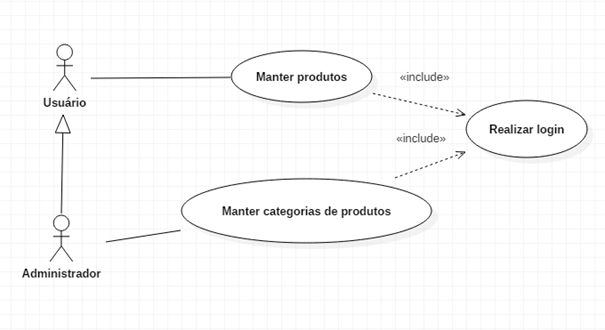
\includegraphics{images/figura2.png}
% 	\end{center}
% 	\caption{\label{fig:Fig_2}Diagrama de casos de uso}
% 	\fonte{Elaborado pelo autor deste trabalho com o uso da ferramenta StarUML (2018).}
% \end{figure}

% O usuário do tipo administrador herda as funcionalidades do usuário comum... 

% Para executar as funcionalidades, os usuários devem realizar o login...

% A documentação dos casos de uso encontra-se no Apêndice A deste trabalho.

% % ----------------------------------------------------------
% \subsection{Modelos de dados}
% % ----------------------------------------------------------

% O modelo de dados é um diagrama que descreve o esquema do banco de dados. Caso o seu projeto utilize este tipo de diagrama, não se esqueça de explicá-lo após a ilustração, conforme o exemplo a seguir.

% \begin{figure}[htb]
%     \begin{center}
% 	    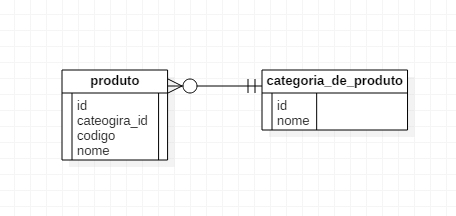
\includegraphics{images/figura3.png}
% 	\end{center}
% 	\caption{\label{fig:Fig_3}Modelo de banco de dados}
% 	\fonte{Elaborado pelo autor deste trabalho com o uso da ferramenta StarUML (2018).}
% \end{figure}

% O esquema de banco de dados é composto de duas tabelas...Os campos do tipo “id” são utilizados para...

% O código SQL de construção do esquema de banco de dados encontra-se no Apêndice B deste trabalho.

% ----------------------------------------------------------
\subsection{IMPLEMENTAÇÃO}
% ----------------------------------------------------------

Nesta seção você pode falar um pouco sobre o código desenvolvido. Não é necessário explicar ou apresentar todo o código fonte da aplicação. Você pode focar nas principais classes ou funções. É importante explicar quais foram as ferramentas utilizadas e o porquê da escolha de cada uma delas.

Você deve colocar o código na pasta sources e carrega-lo ao apêndice, usando aqui apenas uma referência ou trechos de código.

O código presente no Apêndice \ref{apendice:b} representa ....